\documentclass[conference]{IEEEtran}

\makeatletter
\def\ps@IEEEtitlepagestyle{%
  \def\@oddfoot{\mycopyrightnotice}%
  \def\@evenfoot{}%
}
\def\mycopyrightnotice{%
  {\footnotesize XXX-X-XXXX-XXXX-X/XX/\$XX.00~\copyright~20XX IEEE\hfill}%
  \gdef\mycopyrightnotice{}
}
\makeatother

\IEEEoverridecommandlockouts
\usepackage{cite}
\usepackage{amsmath,amssymb,amsfonts}
\usepackage{algorithmic}
\usepackage{graphicx}
\usepackage{textcomp}
\usepackage{xcolor}
\usepackage{tikz}
\usetikzlibrary{arrows.meta,positioning,fit,backgrounds,decorations.pathreplacing}
\usepackage{booktabs}
\usepackage{balance}
% Revision marks: set \revmarkstrue to show changes in red,
% \revmarksfalse for a clean camera-ready copy.
\newif\ifrevmarks\revmarkstrue
\newcommand{\rev}[1]{\ifrevmarks\textcolor{red}{#1}\else#1\fi}

\def\BibTeX{{\rm B\kern-.05em{\sc i\kern-.025em b}\kern-.08em
    T\kern-.1667em\lower.7ex\hbox{E}\kern-.125emX}}

\begin{document}

\title{Hierarchical Behavior Planning for Multi-Robot Systems Based on Large Language Models}

\author{\IEEEauthorblockN{Luc\'ia Petit}
\IEEEauthorblockA{\textit{ETSI Telecomunicaci\'on} \\
\textit{Universidad Polit\'ecnica de Madrid}\\
Madrid, Spain}
\and
\IEEEauthorblockN{Rafael Sendra-Arranz}
\IEEEauthorblockA{\textit{Center for Automation and Robotics} \\
\textit{Spanish National Research Council (CSIC-UPM)}\\
Madrid, Spain}
\and
\IEEEauthorblockN{\'Alvaro Guti\'errez}
\IEEEauthorblockA{\textit{ETSI Telecomunicaci\'on} \\
\textit{Universidad Polit\'ecnica de Madrid}\\
Madrid, Spain}
}

\maketitle

\begin{abstract}
Large language models (LLMs) can interpret heterogeneous information and
select coherent courses of action without relying on hand-coded rules,
 making them attractive as high-level decision modules for robot
teams operating under partial information. However, their inference
latency is incompatible with the time scale of physical control. This
paper presents a hierarchical, hybrid architecture for behavior planning
and generation in multi-robot systems, in which a central LLM converts a
natural-language mission into macro-tasks assigned to individual robots.
A local LLM on each robot decomposes its macro-task into discrete skills
through an observe--reason--act loop, and a physical layer executes those
skills and guaranties robots safety. Deliberation is decoupled from
control by an event-driven synchronization scheme: a model is queried
only when a skill terminates or fails, which removes the stale-decision
problem observed when the LLM is placed inside the control loop. The
architecture is implemented in a physics-based simulator with a 
20B-parameter model served locally and evaluated in a single-robot task-switching
scenario and a cooperative exploration mission with fleets of up to five
robots. The system reaches a success rate of 94.4\% in the single-robot
scenario and 100\% for fleets of two to four explorers, while
collaborative fusion of independent observations reduces the target
localization error by roughly a factor of two.
\end{abstract}

\begin{IEEEkeywords}
multi-robot systems, large language models, task allocation, hierarchical
architectures, embodied reasoning, swarm robotics
\end{IEEEkeywords}

\section{Introduction}

Multi-robot systems distribute a mission across several comparatively
simple agents and therefore offer redundancy, spatial coverage and
graceful degradation that a single platform cannot match
\cite{torreno2017,sun2025}, which makes them natural candidates for
exploration, search and rescue, monitoring and inspection
\cite{brambilla2013}. The central problem is not locomotion but
coordination: deciding which robot should do what, and when, as the team
and the environment evolve.

Multi-robot task allocation (MRTA) has been formalized as an optimization
problem with a mature taxonomy \cite{gerkey2004,korsah2013}, and
self-organized schemes produce robust collective behavior with minimal
communication \cite{krieger2000,obute2022}. Both families share a
structural assumption: the space of relevant situations is enumerated in
advance, as a cost function or as reactive rules. When an unanticipated
state arises, or evidence must be combined in a way that was not encoded,
the system has no principled way to respond.

Large language models (LLMs) offer a complementary capability. Trained on
broad corpora, they generalize well~\cite{brown2020,bommasani2021} and can
reason over a symbolic description of a situation to reach a decision
\cite{wang2023}. In robotics they have grounded instructions in feasible
skills \cite{ahn2022}, produced executable programs \cite{liang2023},
interleaved reasoning with actions \cite{yao2022} and closed the loop
through textual feedback \cite{huang2022}. Their main limitation is
speed: inference on a locally served model takes seconds, orders of
magnitude slower than a control cycle, so any architecture placing an LLM
in the control loop inherits this mismatch.

This paper addresses this mismatch directly. We propose a layered
architecture in which LLMs act strictly as deliberative
modules and not direct actuator commands, and in which deliberation
is triggered by events rather than time. The contributions are: (i) a
two-level LLM hierarchy that separates fleet-level task allocation from
per-robot tactical skill selection; (ii) an event-driven synchronization
mechanism that eliminates decisions made on uninformed observations; and (iii)
an experimental evaluation, on a single-robot scenario and a cooperative
exploration mission, that quantifies mission success, localization
accuracy, and the coordination cost incurred as the fleet grows.

\section{Related Work}

Hierarchical decomposition is not new to multi-robot planning:
hierarchical task networks expand an abstract goal through a library of
methods, and market-based schemes allocate work by bidding against an
explicit utility function~\cite{gerkey2004,korsah2013}. Both are
effective when the tasks and the criteria for comparing them can be
enumerated at design time. The architecture proposed here retains the
hierarchy but replaces the decomposition library and the bidding function
with semantic reasoning, which is what lets a mission be stated in
natural language and revised as conditions change.

Early work on LLMs for embodied agents focused on grounding. SayCan
\cite{ahn2022} combines the semantic plausibility of a candidate skill
with a learned affordance estimate, ensuring the selected action is
executable; Code as Policies \cite{liang2023} instead has the model emit
programs over a fixed API. Both restrict the model to a closed vocabulary
of primitives, an idea we adopt: our models select from an explicit skill
catalog and never invent commands.

A second line concerns closed-loop operation. ReAct~\cite{yao2022}
interleaves reasoning with actions so the model can revise its plan
mid-episode; Inner Monologue~\cite{huang2022} shows that textual feedback
allows replanning without retraining; AutoRT~\cite{brohan2024} adds a
self-verification stage checking a proposal against operational
constraints. Our design borrows the observe--reason--act structure from
the former two and self-verification from the latter. Embodied LLM agents
have since completed long-horizon tasks in unpredictable environments
\cite{monwilliams2025}, confirming that the deliberative role is where
these models add value.

Work targeting teams rather than individual robots is more recent.
LLM2Swarm \cite{strobel2024} equips swarm members with models that reason
and negotiate locally, while LLM-constructed hierarchical trees decompose
a mission into sub-tasks that are then scheduled against each robot's
individual capabilities and constraints \cite{gupta2025}.
\rev{These differ from ours in where the model sits relative to the
control loop. LLM2Swarm reasons peer-to-peer, with no central allocation
stage nor any rule for when a decision may be applied; the
hierarchical-tree planner decomposes once, before execution, after which
scheduling is algorithmic. Ours keeps both levels active throughout ---
a central allocator re-queried at coordination events, per-robot models
at skill termination --- while never consulting either at control rate.
The novelty is thus not the hierarchy but its pairing with an
event-driven schedule.}
The literature consistently identifies latency, hallucination and
grounding as open obstacles \cite{wang2023,nmi2025editorial}. Relative to
these, this paper treats explicitly the temporal boundary between
deliberation and control: tying the query schedule to skill termination
rather than to the clock lets a fleet coordinated by a locally served
\texttt{gpt-oss:20b}~\cite{gptoss} model complete cooperative missions
reliably, at a coordination cost we quantify.

\section{Proposed Architecture}

\subsection{Layered organization}

The proposed architecture is organized hierarchically, from an abstract
goal to motor commands, and is hybrid in that LLM-based deliberative
reasoning is combined with classical reactive control. Four levels of
abstraction are distinguished (Fig.~\ref{fig:arch}). 
The \emph{mission} is the overall objective, stated by the user in natural language. 
\emph{Macro-tasks} are high-level orders assigned to specific robots. 
\emph{Skills} are discrete, finite behaviors selected by a robot's own model.
The \emph{Reactive layer} is where physical actions command actuators.  

\begin{figure}[t]
\centering
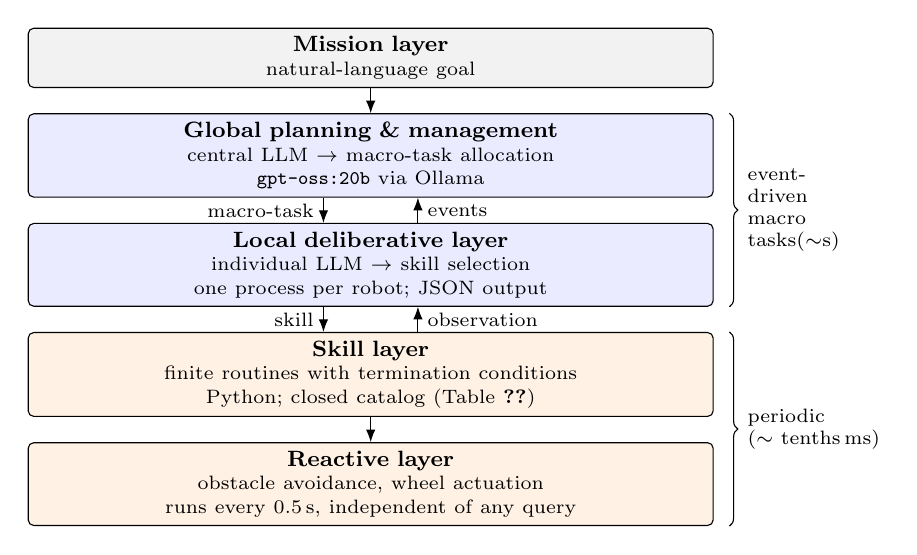
\begin{tikzpicture}[
  font=\footnotesize,
  box/.style={draw, rounded corners=2pt, align=center, inner sep=3pt,
              text width=0.70\columnwidth, minimum height=7.5mm},
  llm/.style={box, fill=blue!8},
  rea/.style={box, fill=orange!10},
  ar/.style={-{Latex[length=1.6mm]}, thin},
]
\node[box, fill=gray!10] (m) {\textbf{Mission layer}\\[-1pt]
  {\scriptsize natural-language goal}};
\node[llm, below=3.2mm of m] (c) {\textbf{Global planning \& management}\\[-1pt]
  {\scriptsize central LLM $\rightarrow$ macro-task allocation}\\[-1pt]
  {\scriptsize\rev{\texttt{gpt-oss:20b} via Ollama}}};
\node[llm, below=3.2mm of c] (l) {\textbf{Local deliberative layer}\\[-1pt]
  {\scriptsize individual LLM $\rightarrow$ skill selection}\\[-1pt]
  {\scriptsize\rev{one process per robot; JSON output}}};
\node[rea, below=3.2mm of l] (s) {\textbf{Skill layer}\\[-1pt]
  {\scriptsize finite routines with termination conditions}\\[-1pt]
  {\scriptsize\rev{Python; closed catalog (Table~\ref{tab:skills})}}};
\node[rea, below=3.2mm of s] (r) {\textbf{Reactive layer}\\[-1pt]
  {\scriptsize obstacle avoidance, wheel actuation}\\[-1pt]
  {\scriptsize\rev{runs every $0.5$\,s, independent of any query}}};

\draw[ar] (m) -- (c);
\draw[ar] ([xshift=-6mm]c.south) -- node[left, pos=0.5, font=\scriptsize]
      {macro-task} ([xshift=-6mm]l.north);
\draw[ar] ([xshift=6mm]l.north) -- node[right, pos=0.5, font=\scriptsize]
      {events} ([xshift=6mm]c.south);
\draw[ar] ([xshift=-6mm]l.south) -- node[left, pos=0.5, font=\scriptsize]
      {skill} ([xshift=-6mm]s.north);
\draw[ar] ([xshift=6mm]s.north) -- node[right, pos=0.5, font=\scriptsize]
      {observation} ([xshift=6mm]l.south);
\draw[ar] (s) -- (r);

\draw[decorate, decoration={brace, amplitude=3pt}]
  ([xshift=2mm]c.north east) -- ([xshift=2mm]l.south east)
  node[midway, right=3pt, font=\scriptsize, align=left]
  {event-\\driven\\ macro\\tasks($\sim$s)};
\draw[decorate, decoration={brace, amplitude=3pt}]
  ([xshift=2mm]s.north east) -- ([xshift=2mm]r.south east)
  node[midway, right=3pt, font=\scriptsize, align=left]
  {periodic\\($\sim$ tenths\,ms)};
\end{tikzpicture}
\caption{Layered architecture. The central LLM converts the mission into
macro-tasks; each robot's individual LLM converts its macro-task into
skills; the skill and reactive layers execute them without further
queries to any model. \rev{Downward arrows carry orders, upward arrows the
events that trigger the next query. Inference runs in a separate process
and exchanges state through a shared blackboard, so the control loop
never blocks on a model.}}
\label{fig:arch}
\end{figure}

The two upper layers are governed by language models. The central model
receives the mission and an aggregated fleet view: identifiers,
sensor values, currently assigned tasks, and a short textual memory --- and
returns an assignment of macro-tasks. This is an MRTA problem posed as
semantic reasoning with a structured output, rather than as an
optimization. The local model on each robot receives its macro-task, a
structured local observation, the last executed skill and its outcome, and
the catalog of available skills, and decides step by step which skill to
run next. Deciding one step at a time, rather than emitting a long
open-loop plan, keeps the sequence adapted to how the environment
actually evolves.

The two lower layers contain no model. Skills are Python routines, each
implementing one behavior and its termination conditions; they translate
intermediate states into actuators commands. Because the model can only name a
skill, its action space is restricted to behaviors that are physically
executable, which bounds the effect of hallucination. The reactive layer
runs inside the fast control cycle, has priority over the deliberative
layers under immediate physical constraints, and remains active even
while a model is being queried.

\subsection{State abstraction and prompting}

Sensors produce high frequency numerical streams, which language models
handle poorly \cite{harnad1990,wang2023}. A pre-processing stage therefore
converts raw readings into \emph{semantic observations} summarizing only
what is relevant for the pending decision, so the model receives a discrete, interpretable state.

Prompts consist of an instruction block --- role, operating rules, the
permitted catalog, and the constraint that no other command may be
emitted --- and a context block with the dynamic information of each
query. Following ReAct \cite{yao2022} the output separates reasoning from action
in JSON, with fields for the reasoning trace, memory and decision. The central model additionally emits a
\texttt{self\_check} block restating the feasibility conditions of its own
proposal, e.g.:

{\footnotesize
\begin{verbatim}
{ "reasoning":..., "memory":...,
  "self_check": {"ready":0, "charging":0,
                 "missing":0, "valid":true},
  "decisions": ["task_robot0", ...] }
\end{verbatim}
}

\noindent The controller validates this block before applying the
assignment, and any decision outside the catalog or violating a mission
constraint is logged as invalid and discarded, the last valid behavior
being retained. Requiring the model to restate the arithmetic of its own
proposal makes inconsistent assignments detectable without a second
query.

\subsection{Failure detection and replanning}

Each skill is a finite process with an explicit termination condition. On
completion the controller emits a semantic observation summarizing the
outcome, acting as a success or failure detector in the spirit of Inner Monolog
\cite{huang2022}, so the model never infers whether an action worked. On failure it receives a semantic explanation ---
orientation not achieved, target already registered, light signal lost
--- and can select an alternative skill rather than repeat the same
one.

\subsection{Event-driven synchronization}

The model is deliberately kept outside the continuous control loop.
Querying it every cycle would let an order computed from stale data
interrupt a maneuver in progress, since inference takes seconds while the
control period is tenths of milliseconds. A new decision is therefore
requested only when the active skill terminates or fails; while a query
is pending the robot holds a \texttt{stop} skill and the reactive layer
keeps it safe. The central model is queried only at coordination moments:
initial planning, completion of a recharge, and final aggregation.

\section{Experimental Setup}

\subsection{Platform}

The experiments were carried out on Mereli \cite{mereli}, a multi-robot
simulator developed at ROBOLABO-ETSIT-UPM, using PyBullet
\cite{pybullet}. Agents are differential-drive robots modeled on the
e-puck~\cite{mondada2009}, with eight-sector proximity and color-specific
light sensors, GPS, compass, and color-differentiated batteries that
discharge while moving and recharge with saturating dynamics near a
beacon \cite{sendra2026}. Reasoning is provided by
\texttt{gpt-oss:20b}~\cite{gptoss} served locally through Ollama
\cite{ollama} via LangChain \cite{langchain}, on a server with an Intel
Core Ultra 7 265K, 93\,GiB of RAM and two NVIDIA RTX 2080 Ti GPUs. Local
inference removes any dependence on external APIs and keeps latency under
experimental control. The model was chosen for its instruction following, well-formed JSON and
respect for the declared catalog. Table~\ref{tab:params} lists the shared
parameters.

\begin{table}[t]
\caption{Common simulation and inference parameters}
\label{tab:params}
\centering
\footnotesize
\begin{tabular}{@{}ll@{}}
\toprule
Parameter & Value \\
\midrule
Simulator / physics engine & Mereli / PyBullet \\
Robot model & e-puck, differential drive \\
Physical time step, $\Delta t$ & 0.05\,s (20\,Hz) \\
Controller period, $T_s$ & 10 steps (0.5\,s, 2\,Hz) \\
Proximity sensor range & 0.8\,m \\
Language model & \texttt{gpt-oss:20b} (local, Ollama) \\
Output format & JSON (reasoning, memory, decision) \\
\bottomrule
\end{tabular}
\end{table}

\rev{No parameter was optimized against the reported metrics. Physical
constants came from the simulator configuration; the controller period
was the slowest rate at which the reactive layer still tracked walls
reliably; the deployment and critical battery levels (0.90 and 0.30) let
a charged robot cross the arena and return. Prompts were developed on
pilot runs excluded from the reported data, and frozen before the
campaign.}

\subsection{Scenario 1: single-robot task switching}

The first scenario validates the local unit in isolation. A single robot
in an arena with light sources and colored ground zones
(Fig.~\ref{fig:arena}a) must sustain a default foraging behavior,
interrupt it to recharge whenever either battery falls below a critical
threshold, and trigger a one-off mission --- switching off three yellow
lights --- once foraging has been ordered a given number of times. The
catalog holds four deliberative skills (Table~\ref{tab:skills}) plus a
reactive obstacle avoider. The prompt states an explicit priority
hierarchy, and the model keeps a short textual memory across queries,
letting it count how often foraging has been ordered and whether the
light mission is complete. Thirty-six runs were executed. \rev{Sample sizes (36 here, 20 per fleet size in
Scenario~2) were set by the cost of local inference, tens of GPU-minutes
per run: the design favors covering five fleet sizes over more
repetitions of one. Proportions carry Wilson 95\%
intervals~\cite{wilson1927}, and smaller differences are not claimed as
effects.} A run succeeds if both batteries stay above zero, the light mission
completes and is resumed after any interruption, and no blocking, timeout
or unrecoverable loop occurs.

\subsection{Scenario 2: cooperative exploration}

The second scenario is the multi-robot extension. A fleet starts on one
side of a square arena with blue battery levels sampled uniformly in
$[0.3, 1.0]$; a blue beacon in the center is the charging station and
fixed red lights are the targets (Fig.~\ref{fig:arena}b). The user states
the mission in natural language, including how many explorers are
required. A robot may only deploy above $0.90$, so the central model must
determine which robots are ready, which must charge and how many are
missing; it is re-queried whenever a recharge completes. The three
central macro-tasks are \emph{wait}, \emph{charge blue battery} and
\emph{search for red lights}; Table~\ref{tab:skills} lists the local
skills into which they decompose.

\begin{figure}[t]
\centering
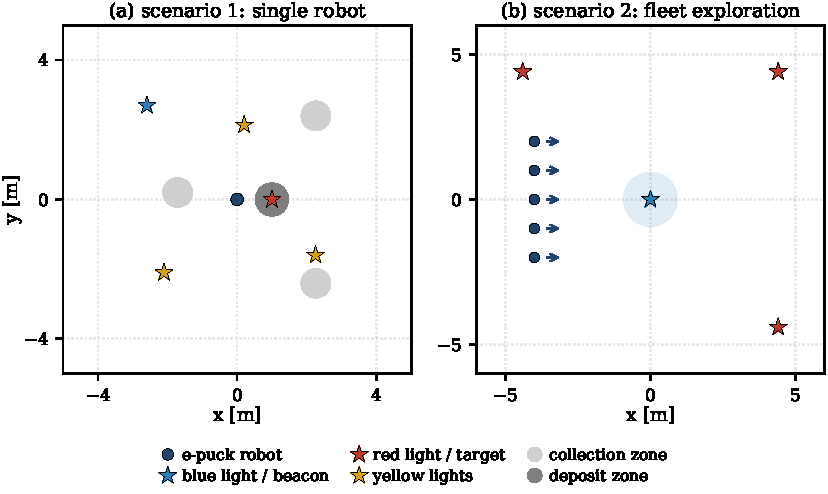
\includegraphics[width=\columnwidth]{figs/arena.pdf}
\caption{Cooperative exploration scenario: the fleet starts on the left,
the blue beacon at the center is the charging station, and the red stars
are the targets. \rev{(a) Metric layout; (b) simulator view. The arena
has no static obstacles beyond its walls and targets are separable by
color --- simplifications discussed in Section~\ref{sec:discussion}.}}
\label{fig:arena}
\end{figure}

\begin{table}[t]
\caption{Local skill catalog in scenarios}
\label{tab:skills}
\centering
\footnotesize
\begin{tabular}{@{}lll@{}}
\toprule
Skill & Function & Termination \\
\midrule
\textbf{Scenario 1} &  &  \\
\texttt{simple\_forage} & Pick and place & new order \\
\texttt{switch\_off\_yellow\_light} & douse light & success / failure \\
\texttt{load\_blue\_battery} & recharge & level $\geq 0.90$ \\
\texttt{load\_red\_battery} & recharge & level $\geq 0.90$ \\
\midrule
\textbf{Scenario 2} &  &  \\
\texttt{stop} & hold position & new order \\
\texttt{navigate} & active exploration & red light detected \\
\texttt{orient\_red\_light} & centre on target & success / failure \\
\texttt{approach\_red\_light} & physical approach & success / failure \\
\texttt{annotate\_red\_light} & spatial registration & completed \\
\texttt{go\_to\_coordinates} & displacement & waypoint reached \\
\texttt{load\_blue\_battery} & recharge & level $\geq 0.90$ \\
\bottomrule
\end{tabular}
\end{table}

Robots never observe the true position of a target. Executing
\texttt{annotate\_red\_light}, a robot records \emph{its own} pose at
detection, with the perceived intensity and simulation step. This
reproduces the error structure of a real deployment, where target
location is inferred from imperfect observations. All reports are then
passed to the central model, which clusters nearby observations and
estimates one position per target; a distance-based fallback covers the
case where the model does not answer in time. Twenty runs were executed per fleet size, from one to five explorers. A
run succeeds if exactly the requested number of ready explorers deploys,
all targets are detected and registered, the aggregated estimate is
produced, and no critical failure occurs.

\section{Results}

\subsection{Single-robot scenario}

The single-robot controller completed 34 of 36 runs, a success rate of
94.4\% with a 95\% Wilson interval $[81.8\%, 98.4\%]$ \cite{wilson1927}.
Of the two failures, one exhausted a battery and the other did not
complete the light mission. The model alternated coherently between
foraging, recharging and the one-off mission, and resumed an interrupted
mission after recharging, confirming that the textual memory suffices to
track progress across queries.

\begin{figure}[t]
\centering
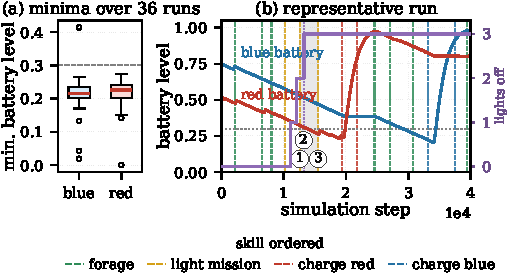
\includegraphics[width=\columnwidth]{figs/singlerobot.pdf}
\caption{Single-robot scenario. (a) Minimum battery level reached per
run. (b) Representative run: both batteries, the cumulative count of
yellow lights switched off, and the skills ordered by the model (dashed
lines). The shaded band spans the stale-decision interval, from the query
at step $12{,}590$ (1) to its application at step $15{,}510$ (3), by which
time the mission had already completed at step $13{,}210$ (2).}
\label{fig:singlerobot}
\end{figure}

Fig.~\ref{fig:singlerobot}(a) reports the minimum level reached by each
battery per run. Medians lie around $0.22$, so recharging normally
triggers with margin, but a few runs approach zero. The cause is latency:
between a level crossing the threshold and the order arriving, several
hundred control steps may elapse, during which discharge continues.
Fig.~\ref{fig:singlerobot}(b) makes the point sharper. A query issued at
step $12{,}590$ (1) correctly ordered the light mission to continue, since
only two lights were off at that time; the answer was applied at step
$15{,}510$ (3), by which point the running routine had switched off the
third light and completed the mission at step $13{,}210$ (2). The decision
was correct for the state observed and obsolete when it took effect, which
motivated the event-driven scheme of the second scenario.

\subsection{Fleet deployment and mission success}

Fig.~\ref{fig:success}(a) shows mission success against the number of
requested explorers. Fleets of two, three and four succeeded in all
twenty runs. The only failures occurred at the extremes: two runs with a
single explorer missed a target, and one with five failed during
deployment. None was caused by an LLM timeout, battery exhaustion or an
unresolved blockage --- errors at the level of individual decisions were
absorbed by subsequent ones, which is what the feedback loop is designed
to produce.

\begin{figure}[t]
\centering
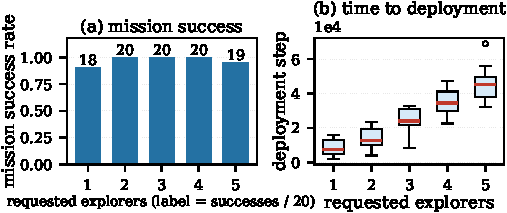
\includegraphics[width=\columnwidth]{figs/success.pdf}
\caption{Mission success rate (a) and number of simulation steps required
to deploy the requested fleet (b), as a function of the number of
requested explorers.}
\label{fig:success}
\end{figure}

Unfortunately, coordination is not free as apreciated in  Fig.~\ref{fig:success}(b), 
which  shows the number of steps needed to reach a correct deployment. 
The median grows monotonically from about $7{,}000$ steps for a single explorer to about
$45{,}000$ for five. The reason is structural rather than computational:
requiring $n$ robots to satisfy the readiness condition simultaneously
makes it increasingly likely that at least one still needs to charge, so
the central model must serialize recharges before the mission can start.

The division of labor between the two levels is visible within
individual runs. Given \emph{charge blue battery}, the receiving robot
does not begin charging directly: its local model first selects
\texttt{go\_to\_coordinates} to reach the beacon, then
\texttt{load\_blue\_battery}. Likewise \emph{search for red lights}
expands into \texttt{navigate}, \texttt{orient\_red\_light},
\texttt{approach\_red\_light} and \texttt{annotate\_red\_light}, driven by
what the robot perceives. Robots not selected hold \texttt{stop} until
activated, so the requested team size is respected exactly. The local
models therefore concretize the order in the light of their own state
rather than echoing it.

\subsection{Detection and collaborative triangulation}

Target detection was essentially saturated: the median detection rate was
$1.0$ for every fleet size, with isolated outliers from the failed runs
above. Coverage is therefore robust to team size in this arena, and the
interesting variable is the accuracy of the aggregated estimate.

\begin{figure}[t]
\centering
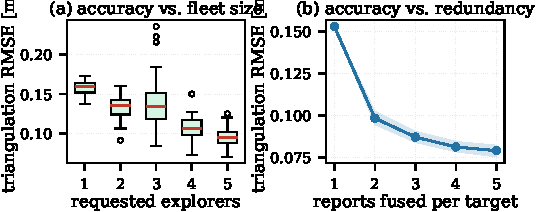
\includegraphics[width=\columnwidth]{figs/rmse.pdf}
\caption{Localisation error of the central estimate. (a) RMSE against
the number of requested explorers. (b) RMSE against the number of
independent reports fused per target, with a 95\% confidence band.}
\label{fig:rmse}
\end{figure}

Fig.~\ref{fig:rmse}(a) reports the RMSE of the central estimate against
fleet size: the error falls from a median of about $0.16$\,m with one
explorer to roughly $0.095$\,m with five. Fig.~\ref{fig:rmse}(b) isolates
the mechanism by conditioning on the number of independent reports fused
per target, irrespective of how many robots were deployed. RMSE drops
from $0.153$\,m with one report to $0.098$\,m with two and $0.079$\,m
with five, the largest gain being from one report to two. This is the
clearest quantitative benefit of the multi-robot setting: cooperation
improves the estimate not only by covering more arena but by supplying
redundant, partially independent evidence about the same target.

\subsection{Decision validity and robustness}

Mission success and decision quality are distinct properties. A run may
complete correctly even if a model produced an invalid answer, provided
the system detects it, discards it and continues with a safe action.
Invalid outputs were of two kinds: malformed JSON, and syntactically
valid answers naming a non-existent action or violating a constraint ---
for instance proposing to deploy a robot whose own \texttt{self\_check}
block reported it as still charging. Both were caught at validation.

\rev{Across the 100 runs of Scenario~2, 225 invalid central decisions
were recorded, growing with fleet size (11, 23, 41, 62 and 88 for one to
five explorers). Self-check contradictions --- assignments inconsistent
with the readiness counts just restated --- account for 218; malformed
JSON (3) and constraint violations (4) occur only at the largest sizes.
The failures are therefore not of format, which the prompt controls well,
but of arithmetic consistency over a longer robot list. Mission success
did not follow: the size with the most invalid decisions (five, 88)
failed once and the fewest (one, 11) failed twice.} This is the practical benefit of
combining a closed action catalog with semantic feedback: an invalid
decision costs one deliberation cycle rather than the mission, because
the next query is issued from an updated state\rev{, and a discarded
decision leaves the robot holding a safe \texttt{stop} skill rather than
acting on a bad order}.

\subsection{Cost of coordination}

The mean central inference latency remained between approximately 25 and
35\,s, rising at five explorers, where the model must reason over more
robots and verify stricter readiness conditions. Local latencies also
grew with fleet size, as more concurrent tactical states must be
resolved.
\rev{Averages, however, hide the tail that matters for control. Local
latency medians rise from $5.5$\,s at one explorer to $21.5$\,s at five
(IQRs $[4.8,7.2]$ and $[13.5,26.4]$\,s), so the architecture becomes not
only slower but less predictable as the fleet grows; central means rise
more gently, from $27.9$ to $35.3$\,s.} With the deployment times of
Fig.~\ref{fig:success}(b), this is a genuine trade-off: additional agents
improve coverage and accuracy but increase deliberative load, deployment
time and the variability of response times.

\rev{Whether this is acceptable depends on the task's time constant. It
suits missions whose decision points are tens of seconds apart ---
exploration, inspection, monitoring --- where a skill runs far longer
than the query that selected it, but not applications needing sub-second
re-planning. The architecture bounds latency's consequence rather than
removing it: obstacle avoidance never waits on a query, so a slow answer
costs mission time, not integrity.}

\section{Discussion}
\label{sec:discussion}

Three observations follow. First, the layered separation is what makes
the system work: because the model selects discrete skills rather than
motor commands, its reasoning is exploited without responsibilities that
demand millisecond responses, and the closed catalog bounds the consequences of an invalid output.

Second, the temporal boundary matters as much as the functional one. A
decision can be correct for the state observed at query time and obsolete
when applied; tying queries to skill termination addresses this
structurally, letting the model operate on a time scale compatible with
its inference cost.

Third, prompt design involves a trade-off. Over-constraining turns the
model into an expensive finite-state machine and discards the flexibility
that motivates its use, while under-constraining produces invalid
decisions. The differential value of the model appeared where explicit
rules are weakest: fusing heterogeneous reports into a single estimate,
and reallocating a fleet in unanticipated states.

\rev{\subsection{Limitations}}

The main limitations are the simulated setting and the latency.
\rev{Three transfer gaps are foreseeable. A real sensor produces false
positives, and an erroneous detection would enter the abstraction layer
as a confident observation and propagate into the fused estimate;
confidence-weighted reporting and cross-robot agreement are the natural
defenses. Exact termination conditions must become tolerance-based, and
odometry drift would degrade the poses triangulation depends on. A radio
link introduces loss and delay the blackboard does not. The layered
structure localizes these risks, but none is exercised here.}

\rev{The evaluation used a single model, so sensitivity to scale remains
open. Two effects compete: smaller models were discarded in development
for inconsistent instruction following, suggesting a floor below which
self-check degrades, while larger ones would raise the latencies above
proportionally.}

\rev{No comparison against a conventional MRTA baseline is reported,
which is a genuine gap: a threshold or auction-based allocator would
very likely deploy the fleet faster than the $27$--$35$\,s central
queries measured here, since the readiness rule of Scenario~2 can be
encoded directly. The comparison this paper cannot yet make is on
missions whose allocation criterion is unknown in advance --- the regime
targeted.}

\rev{Two further constraints apply.} The arena had no static obstacles
beyond its walls, so the reactive layer was exercised mainly by
robot--robot interaction\rev{, leaving its behavior under clutter
untested}. The central coordinator is a single point of failure and the
dominant source of latency\rev{, and the serialization of recharges it
performs drives the growth in Fig.~\ref{fig:success}(b). Three routes
could relax it: decentralized allocation with the central model
arbitrating only conflicts; delegating readiness bookkeeping to a smaller
model; or partial deployment, letting ready robots explore while others
charge}.

\section{Conclusion}

We have presented a hierarchical, hybrid architecture for behavior
planning in multi-robot systems, in which a central language model
allocates macro-tasks over a fleet, per-robot models decompose them into
discrete skills through a reason--act--observe loop, and reactive
controllers execute those skills autonomously. Decoupling deliberation
from control through event-driven synchronization removes the
stale-decision problem that arises when an LLM sits in the control loop.
The architecture achieved 94.4\% success in a single-robot task-switching
scenario and 100\% for fleets of two to four explorers, with localization
error falling by about a factor of two as reports accumulated.
\rev{These findings are established in simulation, with static,
color-separable targets, an uncluttered arena and a single model: they
are evidence that the architecture is sound, not performance guarantees
for a fielded system, and the mission classes it targets remain a
prospect rather than a demonstrated result.} Future work includes
deployment on physical robots, evaluation across model scales, comparison
against conventional task-allocation baselines, and distributing the
coordinator's role to reduce its latency bottleneck.

\section*{Acknowledgment}

This work has been supported by the Grant PID2023-146540OB-C42 funded by MCIN/AEI/10.13039/501100011033, and partially by the European Commission within the SMAUG project (EU Horizon Europe Grant Agreement 10112129) and the AURICA project: Autonomous and Robust Architectures for Intelligence in Adaptive Control (RP2609560188).


\begin{thebibliography}{00}
\bibitem{torreno2017} A. Torreno, E. Onaindia, A. Komenda, and M. \v{S}tolba, ``Cooperative multi-agent planning: A survey,'' \emph{ACM Comput. Surv.}, vol. 50, no. 6, pp. 1--32, 2017.
\bibitem{sun2025} L. Sun \emph{et al.}, ``Multi-agent coordination across diverse applications: A survey,'' \emph{arXiv:2502.14743}, 2025.
\bibitem{brambilla2013} M. Brambilla, E. Ferrante, M. Birattari, and M. Dorigo, ``Swarm robotics: A review from the swarm engineering perspective,'' \emph{Swarm Intell.}, vol. 7, no. 1, pp. 1--41, 2013.
\bibitem{gerkey2004} B. P. Gerkey and M. J. Matari\'c, ``A formal analysis and taxonomy of task allocation in multi-robot systems,'' \emph{Int. J. Robot. Res.}, vol. 23, no. 9, pp. 939--954, 2004.
\bibitem{korsah2013} G. A. Korsah, A. Stentz, and M. B. Dias, ``A comprehensive taxonomy for multi-robot task allocation,'' \emph{IEEE Trans. Robot.}, vol. 29, no. 5, pp. 1295--1312, 2013.
\bibitem{krieger2000} M. J. B. Krieger and J.-B. Billeter, ``The call of duty: Self-organised task allocation in up to twelve mobile robots,'' \emph{Robot. Auton. Syst.}, vol. 30, no. 1, pp. 65--84, 2000.
\bibitem{obute2022} S. O. Obute \emph{et al.}, ``Swarm foraging under communication and vision uncertainties,'' \emph{IEEE Trans. Autom. Sci. Eng.}, vol. 19, no. 3, pp. 1446--1457, 2022.
\bibitem{brown2020} T. Brown \emph{et al.}, ``Language models are few-shot learners,'' in \emph{Adv. Neural Inf. Process. Syst.}, vol. 33, 2020, pp. 1877--1901.
\bibitem{bommasani2021} R. Bommasani \emph{et al.}, ``On the opportunities and risks of foundation models,'' \emph{arXiv:2108.07258}, 2021.
\bibitem{wang2023} J. Wang \emph{et al.}, ``Large language models for robotics: Opportunities, challenges, and perspectives,'' \emph{arXiv:2311.07226}, 2023.
\bibitem{ahn2022} M. Ahn \emph{et al.}, ``Do as I can, not as I say: Grounding language in robotic affordances,'' in \emph{Proc. Conf. Robot Learn.}, 2022, pp. 287--318.
\bibitem{liang2023} J. Liang \emph{et al.}, ``Code as policies: Language model programs for embodied control,'' in \emph{Proc. IEEE Int. Conf. Robot. Autom.}, 2023, pp. 9493--9500.
\bibitem{yao2022} S. Yao \emph{et al.}, ``ReAct: Synergizing reasoning and acting in language models,'' \emph{arXiv:2210.03629}, 2022.
\bibitem{huang2022} W. Huang \emph{et al.}, ``Inner monologue: Embodied reasoning through planning with language models,'' in \emph{Proc. Conf. Robot Learn.}, 2022, pp. 1769--1782.
\bibitem{brohan2024} A. Brohan \emph{et al.}, ``AutoRT: Embodied foundation models for large scale orchestration of robotic agents,'' \emph{arXiv:2401.12963}, 2024.
\bibitem{monwilliams2025} R. Mon-Williams \emph{et al.}, ``Embodied large language models enable robots to complete complex tasks in unpredictable environments,'' \emph{Nat. Mach. Intell.}, vol. 7, no. 5, pp. 592--601, 2025.
\bibitem{strobel2024} V. Strobel, M. Dorigo, and M. Fritz, ``LLM2Swarm: Robot swarms that reason, plan and collaborate through LLMs,'' \emph{arXiv:2409.04163}, 2024.
\bibitem{gupta2025} P. Gupta \emph{et al.}, ``Generalized mission planning for heterogeneous multi-robot teams via LLM-constructed hierarchical trees,'' \emph{arXiv:2501.16539}, 2025.
\bibitem{nmi2025editorial} ``Robot planning with LLMs,'' \emph{Nat. Mach. Intell.}, vol. 7, p. 521, 2025.
\bibitem{harnad1990} S. Harnad, ``The symbol grounding problem,'' \emph{Physica D}, vol. 42, pp. 335--346, 1990.
\bibitem{mereli} Robolabo Research Group, ``Mereli: multi-environment robotics simulator,'' Univ. Polit\'ecnica de Madrid, 2024.
\bibitem{pybullet} E. Coumans and Y. Bai, ``PyBullet: physics simulation for robotics and machine learning,'' 2021.
\bibitem{mondada2009} F. Mondada \emph{et al.}, ``The e-puck, a robot designed for education in engineering,'' in \emph{Proc. ROBOTICA}, 2009, pp. 59--65.
\bibitem{sendra2026} R. Sendra-Arranz, \'A. Guti\'errez, and A. L. Christensen, ``Evolution of transferable self-organized communication modules for swarm robotics,'' \emph{IEEE Trans. Cybern.}, vol. 56, pp. 595--608, 2026.
\bibitem{gptoss} OpenAI, ``gpt-oss-120b \& gpt-oss-20b model card,'' 2025, arXiv:2508.10925 (Apache-2.0; 21B params, 3.6B active).
\bibitem{ollama} Ollama Contributors, ``Ollama: local LLM inference,'' 2024.
\bibitem{langchain} LangChain Inc., ``LangChain,'' 2024.
\bibitem{wilson1927} E. B. Wilson, ``Probable inference, the law of succession, and statistical inference,'' \emph{J. Amer. Statist. Assoc.}, vol.~22, pp.~209--212, 1927.
\end{thebibliography}

\end{document}
